\documentclass[../../../../../../dd.tex]{subfiles}

\begin{document}

	\subsection{Presentation Tier}
		On this tier the two main components that we find are the Web Browser User Interface and the Application User Interface. This two components are different for programming language and it will run on different devices. But, this two component, must comunicate with the controller via the same set of class that must send and read data in the same way. The idea was that the view of the UI can change to be optimized for the device, but the communication with the Logic tier must be the same. So each UI have two kind of classes, the first kind of classes are the classes of visualization that must follow the organization shown on the mock object of the RASD. For example on the RASD we describe all the pages and all the input form of the two kind of application. The second class of classes must contain a class that can sent message to the Logic Tier and one that can receive its responses. We call the first class CommandSender and the second one ResponseReciver.

		\begin{figure}[H]
				\centering
				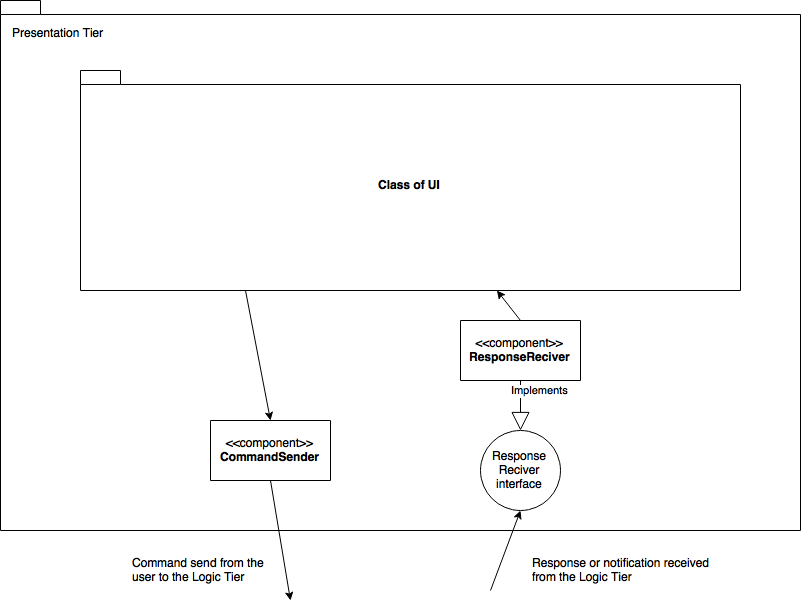
\includegraphics[width=\textwidth, scale=0.5]{../images/PresentationTier.png}
			\caption{Presentation Tier Structure}\label{fig:PresTier}
		\end{figure}
	
\end{document}